\section{Das heirloom-project}
Das heirloom-project wurde 2007 von Gunnar Ritter erstellt und enthält eine Sammlung von traditionellen Unix \textit{Dienstprogrammen}. Die Idee dahinter ist nicht alte Programme zu Verfügung zustellen, sondern nur bestimme Aspekte wie den Stil, Algorithmen oder das \textit{Interface} beizubehalten und für diese einen \textbf{modernisierten \textit{Framework}} zu bieten.

\section{Das Programm cat}
Der Name des Programms cat leitet sich von dem Wort concatenate ab. Dies bedeutet verketten oder verknüpfen. Daraus lässt sich auch schon schließen wo für dieses Programm gedacht ist. Es dient dazu Dateien zusammenzufügen, also dem verketten von Dateien. Häufig wird es allerdings genutzt um sich den Inhalt von Dateien auf dem Terminal auszugeben. Es wird damit eine Verkettung von Datei und Bildschirm erzielt. Dies eignet sich allerdings nur für kleineren Dateien, da sonst das Terminal schnell unübersichtlich wird. Ein guter Verwendungszweck für dieses Programm ist die Verwendung mit zusätzlichen Operatoren, wie dem \textit{Pipe-Operator} um den Inhalt in andere Dateien umzuleiten.

\subsection{Kompilation und Beobachtungen}
Der erste Kompilationsversuch wurde mit dem Kompiler clang ausgeführt. Dazu wurde folgender Befehl genutzt.

\begin{lstlisting}
clang cat.c -o cat.elf
\end{lstlisting}

Allerdings generierte dieser einen Fehler. Dieser ist in Abbildung \ref{clang_cat.c_fehler} zusehen. Es fehlt eine Bibliotheksdatei namens sfile.h .

\begin{figure}[h]
	\centering
	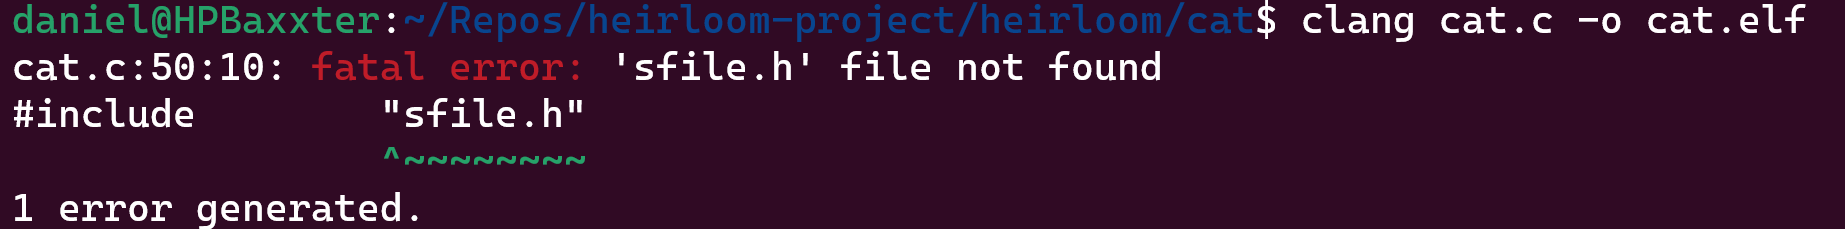
\includegraphics[scale=0.5]{Images/1_clang_cat.c.png}
	\caption{Fehlermeldung beim Versuch die Datei cat.c zu kompilieren}
	\label{clang_cat.c_fehler}
\end{figure}

In einem weiteren Versuch wurde versucht mit gcc zu kompilieren, allerdings führte dies zum selben Ergebnis.

\section{Die Datei cat.1}

\section{Der Programmcode von cat.c}
In diesem Abschnitt wird der Code des Programms cat.c Zeile für Zeile durchgegangen, um nachzuvollziehen was dort geschieht. Dabei wird der Einleitende Kommentar von Gunnar Ritter übersprungen. Dort findet man Copyright Aussagen und Benutzungsrechte.

\subsection{Die Versionsabfrage von Gnuc}
Zu beginn des Codes findet man eine Versionsabfrage von \textit{GNUC}. Diese soll feststellen welche Version des Compilers GNUC auf dem Gerät installiert oder ob dieser überhaupt installiert ist. Ist dieser in der Version höher oder gleich 3 \textbf{und} \textit{GNUC\_minor} höher oder gleich 4, wird der Variable USED über die \textit{Attribut Spezfikation} used zugewiesen.

\begin{lstlisting}
#define USED	__attribute__ ((used))
\end{lstlisting}


